%!TEX root =  main.tex
\appendix
\chapter{Detailed List of Self-Healing Approaches}
\label{ap:approches}

This appendix reports \ldots 

\section{Brun's Self-Adapting Reliability} \label{ap:BurnSelf}
\begin{compactitem}
\item[\textbf{Title}]Self-Adapting Reliability in Distributed Software Systems
\item[\textbf{Author}] 
Yuriy Brun, Jae young Bang, George Edwards and Nenad Medvidovic
\item[\textbf{Reference}] 
\cite{brun_self-adapting_2015}
\item[\textbf{Year}] 
2015
\item[\textbf{Application Domain}] 
Distributed computation architecture
\item[\textbf{Self-Healing steps}] Self-healing steps involved are fault-detecting, diagnosis and recovering
\item[\textbf{Technical Approach}]Iterative redundancy technique
\item[\textbf{Basic Idea}] 
The iterative redundancy algorithm aims to deploy the minimum number of jobs to get a consensus in a correct result. If this does not happen, it iteratively deploys the minimum number of additional jobs until a consensus is reached. 

\item[\textbf{Summary of approach}]
Distributed computing architectures ensure the correct execution of each task through voting: multiple independent computational nodes perform the same task and if the majority of executions agree on a result, a consensus exists, and that result is taken to be the solution of that task. Iterative redundancy tries to optimize the use of computational nodes by distributing the minimum number of jobs that perform the same task required to achieve a desired confidence level in the result, assuming that all the jobs’ results agree. Then, if all jobs agree, the task is completed. However, if some results disagree, the confidence level associated with the majority result is diminished because of the chance that the disagreeing results are correct. The proposed approach then reevaluates the situation and distributes the minimum number of additional jobs that would achieve the desired level of confidence.
This process repeats until the agreeing results sufficiently outnumber the disagreeing results to reach the confidence threshold.


The flow-digram of the iterative redundancy algorithm is given by:
\begin{figure}[H]
\center
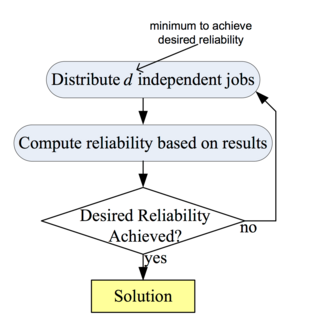
\includegraphics[width=5in]{img/Iterativeredundancyschematic}
\caption{Iterative redundancy schematic:}
\end{figure} 

\item[\textbf{Fault Types}]Byzantine attacks: A Byzantine fault is one where the faulty unit continues to run but produces incorrect results and might lead to failure sometimes. 

\item[\textbf{Failure Types}]Functional failures.

\item[\textbf{Input data}] Results produced by n independent jobs that perform the same task.

\item[\textbf{Recovery actions}]The technique try to  iteratively deploy the minimum number of redundant jobs in order to achieve a consensus on a correct result.

\item[\textbf{Advantages}] Iterative redundancy is more cost effective, than traditional redundancy approaches as it creates the same level of software system reliability at a lower expense.

\item[\textbf{Disadvantages}] In iterative redundancy, the task server deploys several jobs and wait for the responses before possibly choosing to deploy more jobs. Therefore, this technique increases the latency for a particular task.

\item[\textbf{Case studies}]
The technique is implemented and tested on PlanetLab. PlanetLab is a gathering of PCs accessible as a testbed for distributed systems research.\\
\end{compactitem}


\section{SH˜oWA} \label{ap:Showa}
\begin{compactitem}
\item[\textbf{Title}]A Self-Healing Framework for Web-Based Applications (SH˜oWA)

\item[\textbf{Author}]Joao Paulo Magalhaes and Luis Moura Silva

\item[\textbf{Reference}]

\cite{magalhaes_showa:_2015}

\item[\textbf{Year}] 2015

\item[\textbf{Application Domain}]
Web-based applications. 

\item[\textbf{Self-Healing steps}] 
The self-healing steps involved are:Monitor, Plan, Analyze and Execute.

\item[\textbf{Technical Approach}] Statistical correlation (Spearman's rank correlation). 
%The Spearman's rank correlation coefficient (rho) measures the statistical dependence between two variables.

\item[\textbf{Basic Idea}] 
The basic idea is to collect system, application server,
and application-level data, such as response time of per user transactions and CPU time per user transaction, so as to detect and pinpoint anomalies by means of statistical correlation. The performed data analysis detects changes in the server response time and analyses if those changes are correlated with the workload or are due to a performance anomaly. In the presence of performance anomalies, the analysis pinpoints the method calls that are more likely responsible to cause the anomaly.

\item[\textbf{Summary of approaches}] 

The SH˜oWA framework mainly works in four steps. In the first step, SH˜oWA collect system monitor, analyse, plan and execute. Step by step modules consists of various statistical analysis, which are performed during the web application runtime to distinguish performance anomalies from workload variations, to detect the fault and approaching towards recovery procedure. The entire process consists of the following modules (1.sensor module, 2. data preparation module, 3.1. workload variation analysis module, 3.2.performance anomaly analysis module, 3.2.1.anomaly detector module, 3.2.2.root-cause failure analysis module, 4.recovery planner, 5.executor module and 6. effector module)

\begin{figure}[H]
\center
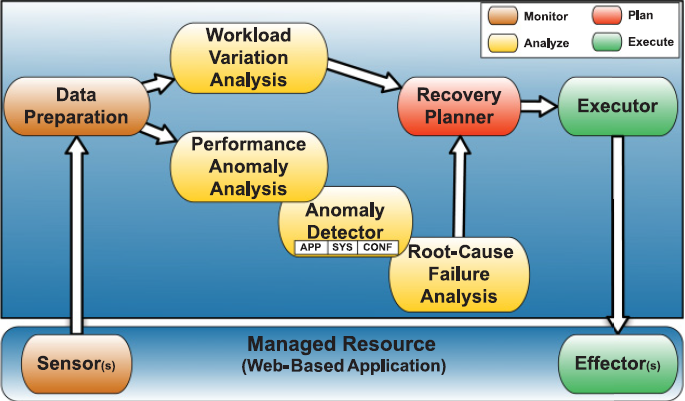
\includegraphics[width=5in]{img/selfhealingframework}
\caption{(SH˜oWA).: self healing framework}
\end{figure}  

The sensor module monitors the system level performance and checks the status of the system services and performance (CPU load, JVM heap memory, number of open files and number of running threads). Additionally, it gathers execution time of application transactions. The data collected by the sensor module gets prepared by the data preparation module, to form an unique key that identifies the various user transactions in the web applications. The prepared data is passed on to the workload variation analysis and performance anomaly analysis modules to detect and pinpoint if any anomaly is present. The data analysis is based on Spearman's rank correlation coefficient represented by rho(p). The correlation coefficient is given by the equation below and it expresses how two variables (X and Y) are associated.

\begin{figure}[H]
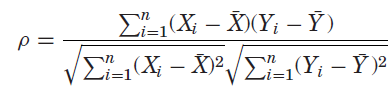
\includegraphics[width=5in]{img/formulae}
\caption{Measure of statistical dependence between two variables.}
\end{figure} 

where X is the sequence of the accumulated response server time per user transaction and Y is the number of user transactions processed in the same interval.If p remains stable and high across the periods of analysis, then it means that the response time is associated with the application workload. If p  decreases, then it means that one of the variables has increased or decreased while the other has remained stable or changed in an opposite direction. This dissociation corresponds to a symptom of performance anomaly.Once the performance anomaly is identified by the Spearman's coefficient equation, the anomaly detector module aims to identify if there is a system or application server changes which is associated with the performance anomaly. For this identification, we create a vector Y for each parameters collected. The vector contains the total number of user transactions precessed in an interval and the accumulated value of the parameters collected by the sensor module in the same interval. If the accumulated value of a given
parameter increases and is not motivated by an increase in the number of requests,then the ρ degree will decrease, showing that a parameter is no longer aligned with the number of requests. The data analysis in this module helps to determine if the application is facing a performance anomaly and verifies if the anomaly is associated with changes in the parameters that has been analyzed by the anomaly detector module. The root cause analysis module analyses user transactions that have only reported a performance anomaly in the previous stage. The root cause analyses module takes two variables X and Y as input and uses the Doane's formulae to determine the exact list of call methods which are creating the response time delay  leading to performance anomaly. Once the list of call methods are identified, the recovery planner module is invoked which contains the recovery procedure for each of the anomalies detected. The recovery procedure is selected according to the type of anomaly detected.In the current implementation, the recovery actions are procedure based and defined by human operator.In future research prospect, it is a novel idea to design the recovery procedures using the machine learning techniques.Once selected, a recovery procedure is executed by the executor module. The main job of the executor module is to execute the specific recovery action which has been triggered with respect to the specific anomaly detected.Once the recovery action has been executed, the handler is passed to the effector module which monitors and keeps track of the number of call methods that has triggered anomaly, how many
of these are in recovery and how any of them has already been recovered.In future research prospect, it is a novel idea to design the recovery procedures using the machine learning techniques.

\item[\textbf{Fault types}]Fail-stutter fault model. 

In fail-stutter fault model, the components of a system sometimes fail and sometimes perform erratically (e.g., low performance) but are not reflected in the final results. These unexpected behaviors are defined as performance faults.

\item[\textbf{Failures types}]Performance failures.

\item[\textbf{Input data}] The input are the parameters which are collected by the sensor module. For instance user transactions, CPU time per user transactions, amount of available memory.

\item[\textbf{Recovery actions}]The output are the recovery strategies which are carried forward or executed against the particular anomalies detected.

\item[\textbf{Advantages}] In SH˜oWA sensor module the monitoring code is separated from the application code, thereby an application can be monitored without the need for manually changing its source code. With this separation, multiple applications can be monitored using the same monitoring code. The framework is generic and can be applied to any type of transactional web application. The only module that needs to be ported is the Sensor module

\item[\textbf{Disadvantages}]The ability to detect anomalies while the number of end users affected is low.
We need the source code of the application to deploy the sensor module.

\item[\textbf{Case studies}]One retail store web application and an auction web application has been used in this paper for testing the framework.
\end{compactitem}



\begin{compactitem}
\item[\textbf{Title}]GenProg: A Generic Method for Automatic Software Repair

\item[\textbf{Author}]
Goues et al.   
\item[\textbf{Reference}]  

\cite{le_goues_genprog:_2012}

\item[\textbf{Application Domain}]
Real, unannotated programs with publicly documented bugs

\item[\textbf{Self-Healing steps:}]. The closed loop repair system works in this way. The method adopts an IDS (intrusion-detection system) that detects the anomalies in the system.

Whenever, the Intrusion Detection System,IDS detects an annomaly, GenProg is invoked to repair the suspicious behavior.

\item [\textbf{Technical Approach}] The method adopts an IDS (intrusion-detection system) that detects the anomalies in the system.

\item[\textbf{Basic Idea}] The program implements three functions:

The \textit{initialpopulation} generates the variants by using the mutual operators based on the input program and test cases.

The \textit{fitness function} evaluates each variants created and chooses the best amongst them.

The \textit{GenProg} iterates by selecting high fitness individuals, which are selected for continuous evolutions for the next.

\item[\textbf{Summary of approach}]
The technical approach used in this paper by the author can be classified in four stages:-
\textit{Program Representation:}Each variant is represented by a pair of an abstract syntax tree   (AST)and a weighted path. The abstract syntax tree contains all the statements of the program and a weighted path contains all the statements in the program that has been assigned a weight based on the occurrence of the statement the test cases.\\

\textit{Selection and Genetic Operators:}GenProg discards individuals with fitness 0 (variants that do not compile or that pass no test cases) and places the remainder in Viable. It then uses a selection strategy to select pop size/2 members of a new generation from the previous iteration.\\ 

\textit{Fitness function:}The fitness function evaluates the acceptability of a program variant. The fitness function mentioned in this paper, encodes software requirements at the test case level: negative test cases encode the fault to be repaired, while positive test cases encode functionality that cannot be sacrificed.\\

\textit{Repair Minimization:}

The search terminates successfully when GP discovers a primary repair that passes all test cases. Due to randomness in the mutation and crossover algorithms, the primary repair typically contains at least an order-of-magnitude more changes than are necessary to repair the program, rendering the repairs difficult to inspect for correctness.


\item[\textbf{Fault Types}]Infinite loop, Segmentation fault, Remote heap buffer over flow to inject code, Remote heap buffer overflow to overwrite variables, Non overflow denial of service, Local stack buffer overflow, Integer overflow and Format string vulnerability.

\item[\textbf{Input data}] Input source code contains a failing negative test case that exercises the defect and a set of passing positive test cases that describe requirements.

\item[\textbf{Recovery actions}]The recovery action is the primary repair that passes all test cases.

\item[\textbf{Advantages}] 
The GP search space focuses genetic operations along a weighted path and takes advantage of test case coverage information, and reusing existing program statements.

\item[\textbf{Disadvantages}] GenProg relies on test cases to encode both an error to repair and important functionality. GenProg cannot repair race conditions as it is difficult to encode an error using test cases for non-deterministic properties.


\end{compactitem}



\begin{compactitem}

\item[\textbf{Title}]Exception Handling for Repair in Service-Based Processes

\item[\textbf{Author}]Friedrich et al.

\item[\textbf{Reference}] 

\cite{friedrich2010exception}

\item[\textbf{Year}] 2010

\item[\textbf{Application Domain}]
Service-based processes

\item[\textbf{Self-Healing steps}] The self healing loop is: design, diagnosis, repair


Diagnosis: This phase determines where the error took place and what the cause of the error is. The knowledge about the fault is crucial for repairing the process and for minimizing the need for re executing parts of the process. Such knowledge is obtained through diagnosis,  using a diagnosis tool.

\item[\textbf{Technical Approach}]Model based approach

\item[\textbf{Basic Idea}] In this paper, we design repair strategies based on the structure of the process by using model-based approach. The repair plan / actions is defined in the process model. The approach is based on the concept of self-healing system. In this approach, the repair information is associated with a process at design time and the repair plans are generated at runtime.

\item[\textbf{Summary of approach}]

\item[\textbf{Fault Types}]The two types of faults that can be healed in this case are: 

\item[\textbf{Failure Types}]The two types of faults that has been healed in this case are:

An incorrect item code with an item name. The system send a wrong shipping note to warehouse, which therefore does not process the order and the package correctly.


When the are house receives the item description from the SHOP through the FORWARDORDER operation, it discovers that the order goods, the shipping note and the package are inconsistent with respect to the goals provided by the supplier and thus raised failure 1.

\item[\textbf{Input data}] 

\item[\textbf{Recovery actions}]

\item[\textbf{Advantages}] 
Repair follows the same logic as the original process and different repairs can be proposed for different causes of failures, with the goal of minimizing both the amount of work to be redone in the process and the compensation and/or reexecution of external services.

\item[\textbf{Disadvantages}] 



\item[\textbf{Case study}] 


The approach has been used on a food shop selling company, which sells products online using a service-oriented architecture (SDA) infrastructure with four services.

\end{compactitem}




